
\section{Introduction}

In today's competitive environment it is essential to get products out in the market as early as possible to capitalize on the first-mover's advantage. Time from idea-to-market is reducing dramatically. To cater to rapid product development, simulation-analysis is performed earlier in the design rather than towards the end, at the testing-validation stage.  Earlier in design, analysis need not be very accurate but has to be quick so as to evaluate various design alternatives. Here a detailed CAD model is not necessary but a more simplified-idealized one is analyzed. Small-irrelevant details add to complexities in mesh generation, and need more resources in terms of computational power-time for a relatively smaller gain in the accuracy of the results. Models are simplified in such a manner that they retain the important details and eliminate the irrelevant ones. This process of conversion from a  detailed model to a simplified one is known as Model Simplification (Figure \ref{ModelSimplification}). Even today it is time-consuming and largely a manual process \citep{Russ2012}. 

Research in the domain of Model Simplification is going on for decades now. As elaborated by Thakur et. al. \citep{Thakur2009} there have been many attempts to automate the simplification process so far. However, at present, only limited capabilities exist for practical usage\citep{Lee2009} .
	
%	\begin{wrapfigure}{l}{0.6\textwidth}
%	\centering
%	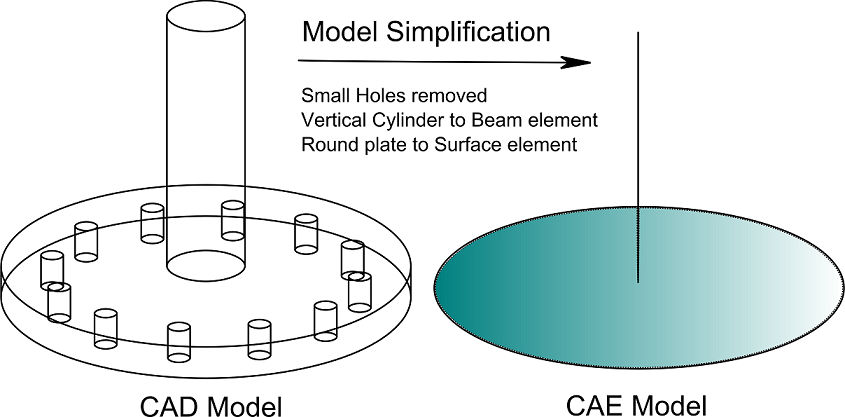
\includegraphics[scale=0.4]{..//Common/images/ModelSimplification.png}
%	\caption{Model Simplification}
%	\label{ModelSimplification}
%	\end{wrapfigure} 

	\begin{figure} [h]
		\centering
		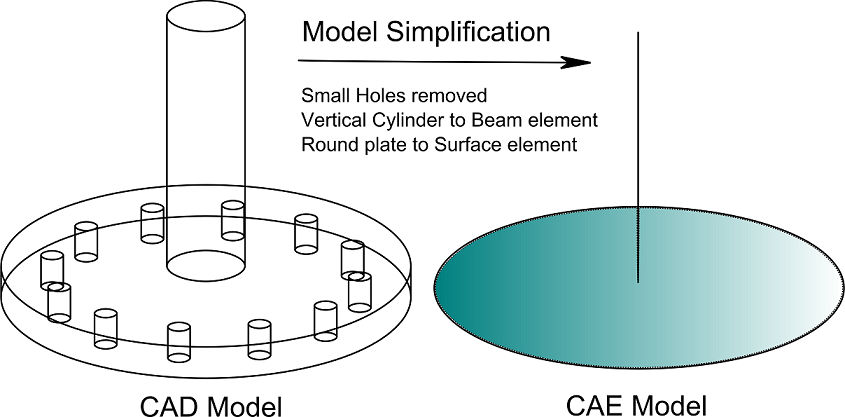
\includegraphics[scale=0.7]{..//Common/images/ModelSimplification.png}
		\vspace{\abovecaptionskip}
		\caption{Model Simplification consisting of both Global and Elemental idealization}
		\label{ModelSimplification}
	\end{figure}

\vspace{-.6cm}

	Model Simplification, according to Dabke \citep{Dabke1994}, can be broken down into two phases, Global and Element Idealization. Global Idealization (also referred as 'de-featuring') deals with suppressing irrelevant features taking advantage of the symmetry to analyze only a portion of the model. In Element Idealization (also referred to as 'idealization'), shapes like slender-bar, thin-wall are converted to lower dimension geometries.

	Many Model Simplification  approaches do not utilize feature information available in the CAD models. They work on the final shape and while doing so, connection of the analysis geometry with the modeling features, relationships and constraints defining the design model, are lost \citep{Smit2011}.
